\section{Descriptive Methods of Data}
After doing the research, we have to represent data in a clear and efficient way. In order to do that, we have \textbf{Descriptive Methods of Data}.\\\Index{Raw Data}: Lots of useless number that need to be sorted.\\

\begin{objectives}
    \item Learn how to describe data with numbers
    \item Know different types of graphs
    \item Know advantages and drawbacks of graphs
    \item Know different experiment error and how they are created
\end{objectives}
\subsection{Graphical Descriptive Methods}
\begin{description}
    
    \item[Graphical]:To describe data with Graphs, it is clearer and easier to attain 
    \begin{description}
        \item[Bar Chart]:It is used to compare value easily and clearly. It can have \textbf{Cluster} where high bars gather and \textbf{Gap} where low bars gather.
        \begin{figure}[H]
            \centering
            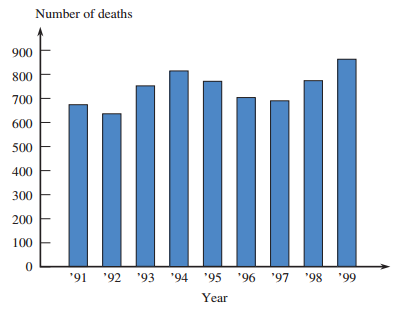
\includegraphics[width=75mm]{bar_chart.png}
            \caption{Bar Chart}
            \label{bar chart}
        \end{figure}
        \item[Dot Plot]: It is used to see which values have the most frequency or the most frequent value of results as well as the distribution of data.
        \begin{figure}[H]
            \centering
            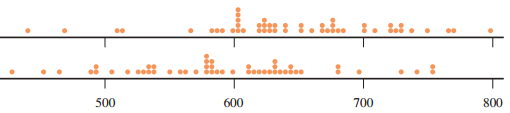
\includegraphics[width=75mm]{dotplot.png}
            \caption{Dot Plot}
            \label{dot plot}
        \end{figure}
        \item[Pie Chart]: It is used to see \textbf{Relative Frequency} or the proportion of different parts.
        \begin{figure}[H]
            \centering
            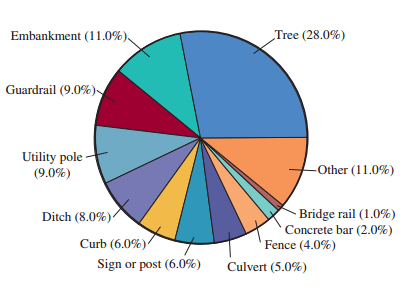
\includegraphics[width=75mm]{pie_chart.png}
            \caption{Pie Chart}
            \label{pie chart}
        \end{figure}
        \item[Segmented Bar Chart]: The same as \textbf{Pie Chart}, just in the form of a bar.
        \begin{figure}[H]
            \centering
            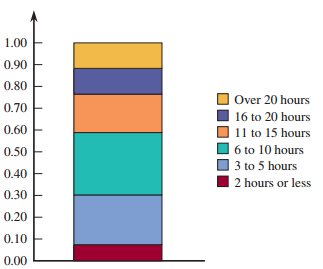
\includegraphics[width=75mm]{segmented_bar_chart.png}
            \caption{Segmented Bar Chart}
            \label{segmented bar chart}
        \end{figure}
        \item[Ogive]: It is used to show the \textbf{Cumulative Frequency}.
        \begin{figure}[H]
            \centering
            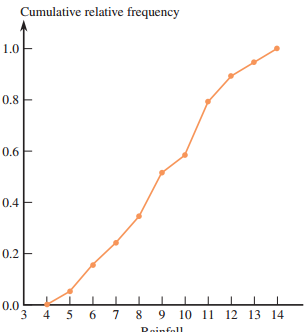
\includegraphics[width=75mm]{crf.png}
            \caption{Ogive}
            \label{crf}
        \end{figure}
        \item[Parete Chart]: The Ogive on the top of the Bar Chart.
        
        \item[Stem and Leave]: It is like a kind of \textbf{Side-way Dot-plot}, can be used to see the distribution of results.
        \begin{figure}[H]
            \centering
            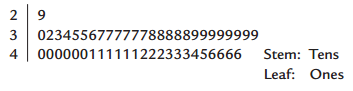
\includegraphics[width=75mm]{stem_leaf.png}
            \caption{Stem and Leaf}
            \label{fig:my_label}
        \end{figure}
        \item[Histogram]: It can be used to show the distribution of data on different \textbf{Class Intervals} which can be \textbf{Continuous or Discrete}.
        \begin{figure}[H]
            \centering
            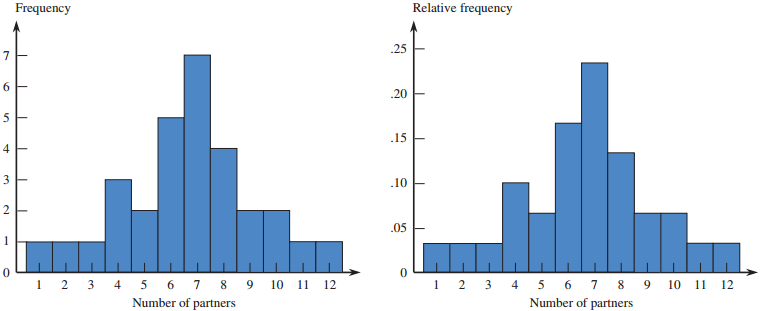
\includegraphics[width=75mm]{histogram.png}
            \caption{Histogram}
            \label{histogram}
        \end{figure}
        \begin{figure}[H]
            \centering
            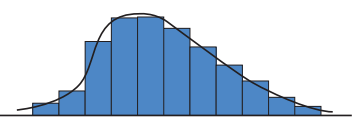
\includegraphics[width=75mm]{smoothed_histogram.png}
            \caption{Smoothed Histogram}
            \label{smoothed histogram}
        \end{figure}
        \item[Box and Whiskers Plot]: It can show the distribution by Right or Left the tail's skewed to.
        \begin{figure}[H]
            \centering
            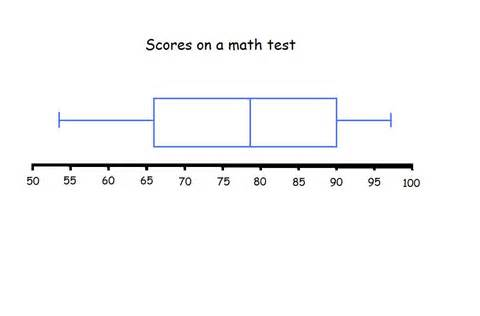
\includegraphics[width=75mm]{th.jpg}
            \caption{Box and Whiskers}
            \label{box and whiskers}
        \end{figure}
        \begin{Question}
            How can Box and Whiskers plot be drawn to a Smooth Histogram
            \solution The narrower the 25 percent, the higher the curve
        \end{Question}
        \item[Scatter Plot]: It can be used to show \textbf{Trends} or \textbf{Correlation} of two factors.
        \begin{figure}[H]
            \centering
            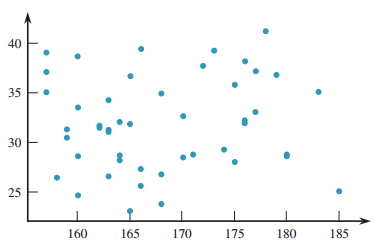
\includegraphics[width=75mm]{scatter.png}
            \caption{Scatter Plot}
            \label{scatter plot}
        \end{figure}
       
        \item[Comparative Bar Chart]: If there are Multiple Samples of \textbf{Categorical Data}.
        \begin{figure}[H]
            \centering
            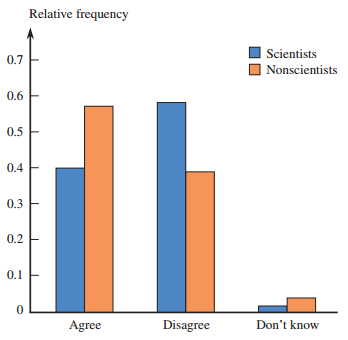
\includegraphics[width=75mm]{comparative_bar_chart.png}
            \caption{Comparative Bar Chart}
            \label{comparative bar chart}
        \end{figure}
    \end{description}
\end{description} 

\subsection{Numerical Descriptive Methods}
Besides using Graphs to represent data, it's also important to know how to describe a data list with numerical descriptive methods to show the features of data clearly and directly.
\begin{itemize}
\item \Index{Describing the Center} When describing numerical data, it is common to report a value that is representative
of the observations. Such a number describes roughly where the data are located or “centered” along the number line, and is called a measure of center. The two most widely used measures of center are the \Index{Mean} and the \Index{Median}.
\begin{itemize}
    \item \textbf{Mean}: The mean of a numerical data set is just the familiar arithmetic average: the sum of the observations divided by the number of observations.
    \begin{equation}
        \bar x=\frac{\Sigma x}{n}
    \end{equation}
    \item \textbf{Median}: Once the data values have been listed in order from smallest to largest, the median is the middle value in the list, and
it divides the list into two equal parts. 
    \item \Index{Mode}: Mode sometimes is used. It is the value that appears in the data set the most often.
\end{itemize}

\item \Index{Describe the Variability}It is also
important to describe how much the observations differ from one another. 
\begin{itemize}
    \item \Index{Range}: The simplest numerical measure of variability is the range. range is the difference between the largest observation and the smallest observation.
    \item\Index{Variance and Standard Deviation}: The customary way to prevent negative and positive deviations from counteracting one another is to square them before combining.
    \begin{equation}
        s_x = \sqrt {\frac{1}{N}\sum\limits_{i = 1}^N {\left( {x_i - \bar x} \right)^2 } }
    \end{equation}
    Variance is just without the square root.
    \item\Index{Interquartile range}: IQR, The difference between the lower quartile and the upper quartile.
    \item \Index{Percentile}: is the median of half of the data set. \Index{Lower quartile Q1}is the median of the lower half, and the \Index{Upper quartile Q3} is the median of the upper half.
\end{itemize}
\end{itemize}
\begin{Question}:
    Do these values count the out-liners?
\end{Question}
\vfill
\newpage



